\documentclass{subfiles}
\begin{document}
\section{Optimization of the Morse Double-Well Parameters}\label{sec:optimization_result}
Applying the optimization procedure outlined in Section \ref{sec:optimization_procedure}, we identify two sets of optimal parameters for the Morse doubl well potential that meet the desired energy and entanglement criteria. Configuration $C_I$ is tailored to yield distinct, well-separated single-particle energy spectrums and vanishing two-body entanglement, while configuration $C_{II}$ is designed to produce a significant two-body entanglement and enforce a degeneracy of the first excited single-particle energy levels in each well to enable coherent mixing of the $\ket{10}$ and $\ket{01}$ logical states.
\\ 

Table \ref{tab:optimized_params} summarizes the five optimized parameters - depths of the left and right wells $D_L$ and $D_R$, widths $k_L$ and $k_R$, and inter-well separation $d$ -  for each configuation, all in atomic units (a.u.). In $C_I$ a deeper left well ($D_L = 73.4060$ a.u.) alongside a shallower right well ($D_R = 71.1004$ a.u.) ensures disctint eigenenergies and a von Neumann entanglement entropy of $S_{VN} = 0.0000$\textcolor{red}{TODO: Calculate, and insert} between the two first excited logical states $\ket{10}$ and $\ket{01}$, confirming a product state regime. Configuation $C_{II}$, on the other hand, slightly increases the right-well depth ($D_R = 71.9918$ a.u.) and adjust a more balanced width for both wells ($k_L = 29.1615$ a.u., $k_R = 29.1677$ a.u.) so that the first excited single-particle energies coincid within numerical tolerance, and we have degeneracy in our two-particle system.

This engineered degeneracy creates a sharp 'entanglement peak' in the potential parameter space, allowing our ramp protocol to traverse from $C_I$ to $C_{II}$ to induce mixing of the logical states $\ket{10}$ and $\ket{01}$, and thus, generate a significant two-body entanglement. The two configuations are similar within a few atomic units, so quantum control protocols can perturb our system without having to significantly alter the systme architecture, with minimal control overhead. \\

These two parameter configuations form the foundation for all subsequent static analyses and dynamical simulations in the thesis work. \textcolor{red}{TODO: Change to the proper parameters, remember to also change the plots showcasing the populations of th states in either configuration. ALSO: Remove remark that this is the only paramters used, in the 2 level system we have separate parameters. Should we add these also here? Or make separate sections? Could give smoe useful insights how the parameters must chang when higher order terms are included. ALSO: Add a discussion on the implications of these parameters for the physical realization of the system, and how they relate to experimental setups. What does this mean for the distance between the particles, and how does this affect the entanglement generation? Are we within working ranges of experimental setups? Other physical properties and constraints that might be relevant at this distance?}
\begin{table}[h!]
  \centering
  \caption{Optimized Morse potential parameters for configurations \(C_1\) (separable) and \(C_2\) (degenerate).}
  \label{tab:optimized_params}
  \begin{tabular}{lcc}
    \toprule
    Parameter & \(C_1\) & \(C_2\) \\
    \midrule
    \(D_L\) (depth of left well)       [a.u.] & 73.4060 & 73.4469 \\
    \(D_R\) (depth of right well)      [a.u.] & 71.1004 & 71.9918 \\
    \(k_L\) (width of left well)       [a.u.] & 31.6126 & 29.1615 \\
    \(k_R\) (width of right well)      [a.u.] & 26.5751 & 29.1677 \\
    \(d\)   (inter-well separation)     [a.u.] & 42.4701 & 42.7983 \\
    \bottomrule
  \end{tabular}
\end{table}

\\ \\ Figure \ref{fig:state_populations_I} show the decomposition of the six lowest two-particle energy eigenstates in the Sinc-DVR product basis for configuration $C_I$, where we observe that the states are indeed pure product states within a numerical tolerance of $10^{-7}$. Each eigenstate has exactly one dominant block, and is zero elsewhere - meaning the there is vanishing two-body entanglement between the particles, as seen from the listed entropy $S$ for each state - just what we aimed to achieve for the separable configuration. 
\begin{figure}[h!]
    \centering
    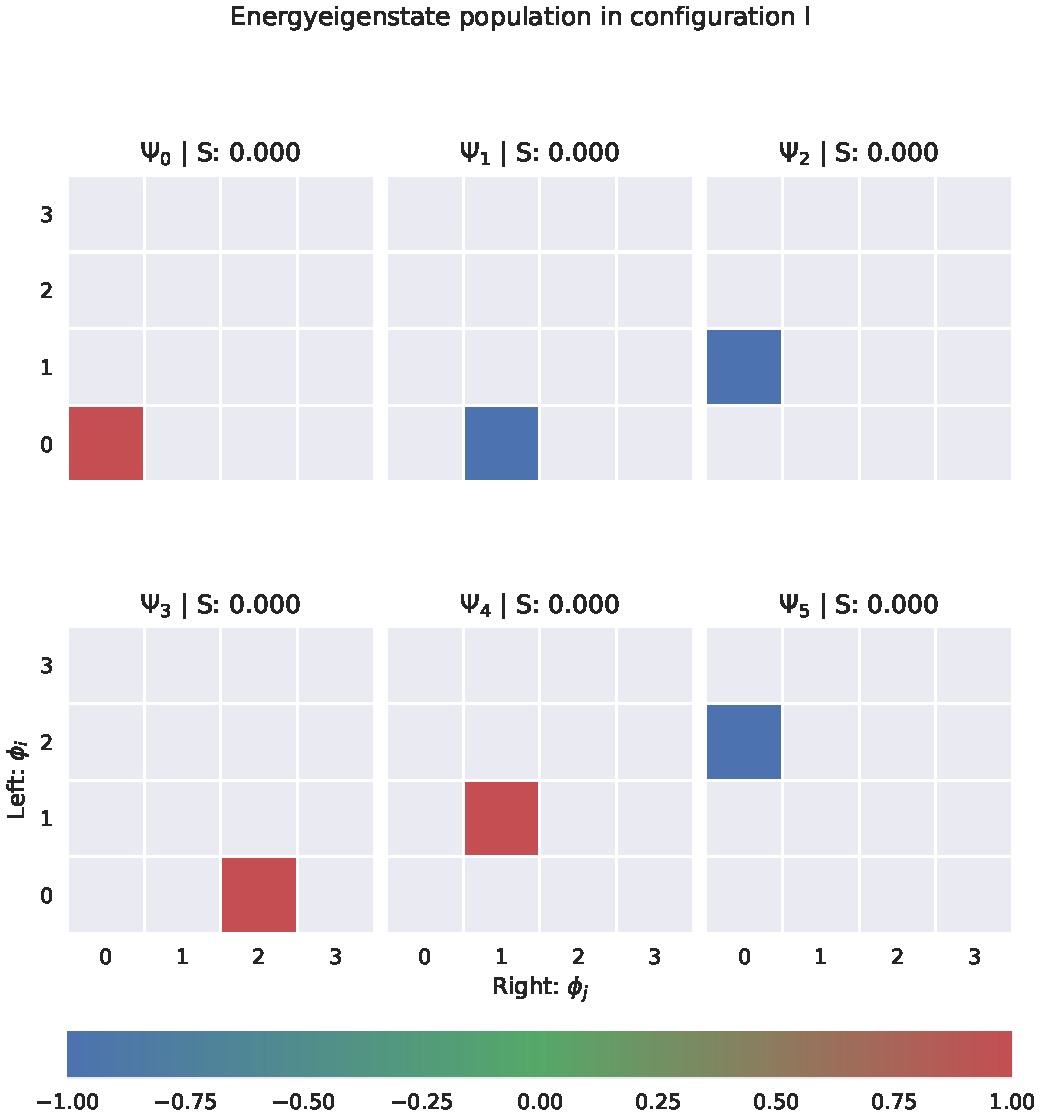
\includegraphics[width=1.0\textwidth]{figs/state_populations_I.pdf}
    \label{fig:state_populations_I}
\end{figure}
\textcolor{red}{TODO: Add discussion on these results. Calculate the tranformation from atomic units to real SI units to quantify what the distance mean. What does this distance impose on the physical realisation of our system? Are we within working ranges of experimental setups? Other physical properties and constraints that might be relevant at this distance?}

\\

By contrast, Figure \ref{fig:state_populations_II} illustrates the same six two-particle energy eigenstates under configuation $C_{II}$, where we observe that the first excited states $\ket{10}$ and $\ket{01}$ are now mixed, with both states having significant contributions from both wells. The mixture is almost equal, and we are close to achieve the Bell states (maximally entangled states) for these two energy eigenstates, as indicated by the entropy $S \approx 1$. This means we have near perfect superpositions of the logical states $\ket{10}$ and $\ket{01}$. The remaining states remain essentially pure product states up to numerical tolerance ($10^{-7}$), highlighting that only the desired qubit subspace is affected by the entanglement, while the rest of the two-particle Hilbert space remains unaffected. This will be crucial for quantum control protocols we aim to run.

\begin{figure}[h!]
    \centering
    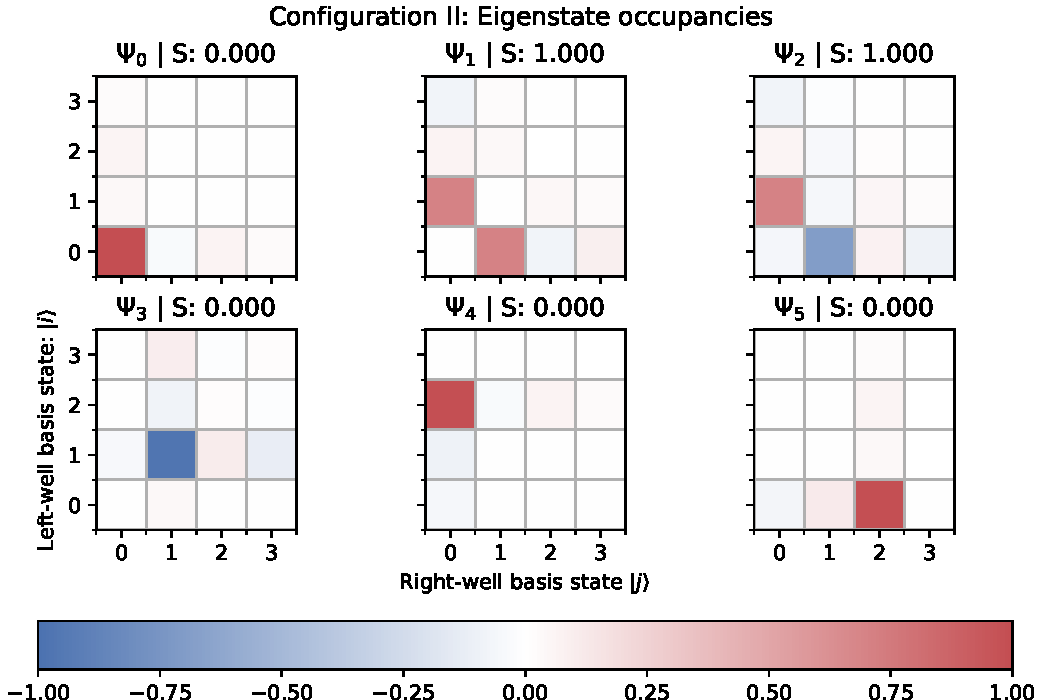
\includegraphics[width=1.0\textwidth]{figs/state_populations_II.pdf}
    \label{fig:state_populations_II}
\end{figure}
\\ \\

Together, these two static heatmaps validate our optimization procedure: Configuration $C_I$ produces well-separated, unentangled energy eigenstates, while configuration $C_{II}$ enforces a degeneracy of the first excited states, enabling a coherent mixing of the logical states $\ket{10}$ and $\ket{01}$, thus generating significant two-body entanglement needed for our two-qubit gate operation protocols. The optimized parameters for both configurations are used in all subsequent analyses and simulations throughout the thesis, ensuring a consistent and controlled environment for our investigations into quantum control and entanglement dynamics in the Morse double-well potential.

\end{document}